\documentclass[12pt,a5]{bxjsarticle}

\usepackage{xltxtra}
\setmainfont{IPAPMincho}
\setsansfont{IPAPGothic}
\setmonofont{IPAGothic}
\XeTeXlinebreaklocale "ja"

\usepackage{hyperref}
\usepackage{listings}
\usepackage{verbatim}

\newcommand{\e}{\mathrm{e}}

\title{物理学情報処理論2 problem5}
\date{}

\begin{document}
\maketitle

\section{}
平面内での散乱。symplectic法にて時間発展させて軌道を描いた。

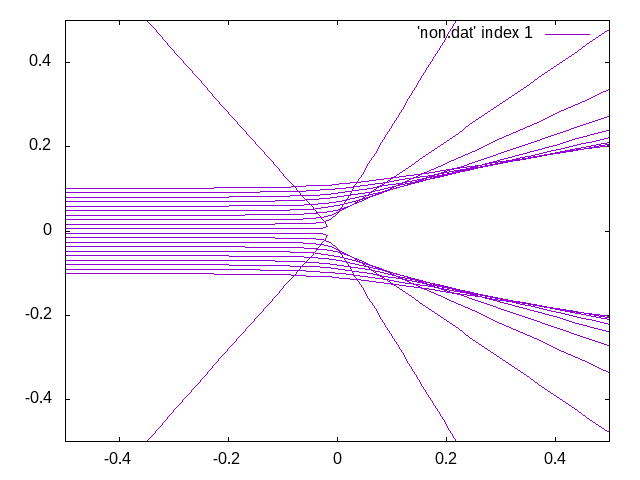
\includegraphics[width=\linewidth]{orbit.png}

相対論を考慮して計算すると以下のような軌道となる。

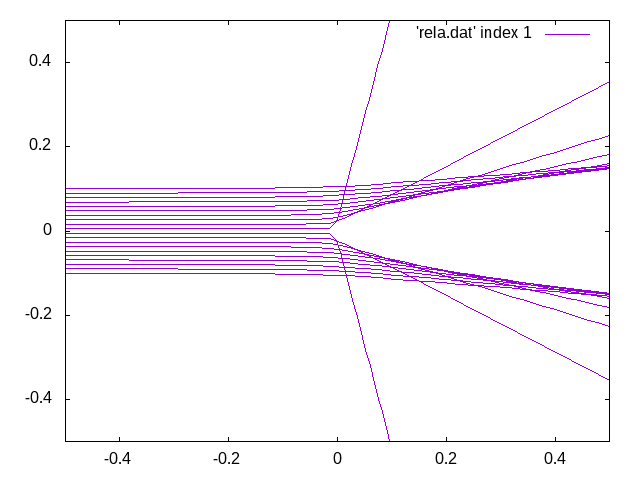
\includegraphics[width=\linewidth]{rela-orbit.png}

これは直感的には相対論を考慮すると、同じ初期条件でもより多くの運動量を持っているということになるため、軌道を変えられづらくなっていることが表われている。

線をそれぞれ分けなくても良いのは、$ -0.5 < x < 0.5, -0.5 < y < 0.5 $の範囲では端は切れてしまうため、
まとめてしまっても大丈夫であるため。

以下のスクリプトを用いて、orbit.datから図を生成した。
\lstinputlisting[caption=plot.sh,language=bash]{plot.sh}

\end{document}
